\chapter{Introdução}

Em outubro de 2023, Manaus destacou-se como a cidade com a pior qualidade do ar no mundo, registrando, em alguns dias do mês, a presença 
de densas nuvens de fumaça. Segundo a prefeitura da capital amazonense, a situação é resultado da 
intensa onda de queimadas na região \cite{G1-ar-manaus}. Portanto, uma preocupação relevante 
é a intoxicação por inalação de gases asfixiantes, como, por exemplo, o monóxido de carbono (CO). O gás, presente no ar devido à combustão 
incompleta de materiais ricos em carbono, é uma substância tóxica, incolor e inodora, que atua no organismo da 
seguinte forma: ao se ligar quimicamente à hemoglobina, proteína no sangue responsável pelo transporte de oxigênio, com uma afinidade de 
200 a 300 vezes maior que a ligação do oxigênio ($O_{2}$), o monóxido de carbono reduz a eficiência do transporte de oxigênio no organismo e 
pode levar a óbito caso haja exposição prolongada e em altas quantidades \cite{carbon-monoxide-poisoning-varon}.

No ambiente doméstico, as fontes mais comuns do gás CO são: aquecedores, fogões, automóveis 
em garagens pouco ventiladas, entre outros. Outro fator de risco é o vazamento devido ao mau 
uso e/ou à falta de manutenção dos equipamentos, pois a detecção do gás antes do início dos 
sintomas é prejudicada na ausência de equipamentos de medição \cite{bio-sufocantes-hernandez2022}. Portanto, 
decidiu-se abordar a problemática por meio de um sistema embarcado, com foco na emissão de 
alerta de risco aos ocupantes. O projeto de trabalho de conclusão de curso consiste na elaboração e 
desenvolvimento de um protótipo de \textit{hardware}, em conjunto com o \textit{software} necessário na 
interação do usuário com os outros módulos do sistema. 

\section{Objetivos}

O objetivo geral do trabalho é oferecer uma solução de sistema embarcado para o monitoramento da qualidade do ar em ambiente residencial, com 
ênfase na coleta de dados e identificação de condições de risco, pois proporcionar aos moradores informações cruciais sobre o estado atual do ar interno 
contribui na adoção de medidas preventivas.

Portanto, para alcançar o objetivo geral, é necessário cumprir os seguintes objetivos específicos:
\begin{itemize}
    \item Elaborar pesquisa com potenciais usuários e realizar avaliação do sistema;
    \item Coletar, compreender e tratar as informações dos sensores de: monóxido de carbono, temperatura e umidade do ar;
    \item Construir o protótipo do dispositivo embarcado;
    \item Realizar a comunicação entre o dispositivo e os demais módulos da aplicação;
    \item Desenvolver a API de dados e eventos, assim como a interface do sistema com o usuário;
\end{itemize}

\section{Justificativa}

O projeto visa contribuir para o monitoramento e detecção de riscos de intoxicação de gás em residências, cujo 
impacto se manifesta na prevenção de acidentes, tomada de decisão com apoio de dados e também na automatização 
de sinais de alerta. Outro ponto de destaque da importância desse trabalho diz respeito ao risco de morte por asfixia 
que a substância monóxido de carbono possui, pois sua presença não é detectada pelo olfato humano e o tempo de exposição é um 
fator determinante para os efeitos na saúde. 

A diminuição no fornecimento de oxigênio causa consequências graves ao organismo, indo desde sintomas brandos como náusea e dores de 
cabeça até casos mais sérios como, por exemplo, lesão neurológica e disritmia cardíaca \cite{carbon-monoxide-poisoning-varon}. Esta perspectiva enriquece a 
contribuição do trabalho no campo de IoT e ressalta a importância do uso de sistemas inteligentes para o monitoramento ambiental.  

\section{Metodologia}

A metologia de trabalho baseia-se no \textit{embedded design life cycle diagram} \cite{system-design-IOT}. O fluxo de atividades possui vantagem no 
particionamento de tarefas em \textit{hardware} (HW) e \textit{software} (SW), pois 
a execução de  múltiplas tarefas no mesmo projeto é positivo para sistemas embarcados e 
suas características intrínsecas, como alto acoplamento, dependência entre componentes eletrônicos e a leitura de dados pelo software, além da própria limitação de 
poder computacional oferecido pelos dispositivos. A execução simultânea de atividades em 
duas áreas permite a validação de funcionalidades do sistema nas entregas incrementais e otimização do 
processo de desenvolvimento, porém sua complexidade exige um cuidado maior com a execução e ordem de tarefas. Portanto, o método original possui 7 fases principais:  

\begin{enumerate}
    \item Especificação do produto;
    \item Particionamento em componentes de \textit{hardware} e \textit{software};
    \item Iteração e refinamento das funcionalidades;
    \item Atividades de \textit{hardware} e \textit{software};
    \item Integração de componentes;
    \item Testes de aceitação e lançamento do produto;
    \item Manutenção e atualização do produto final;
\end{enumerate}

Contudo, o método original trata do desenvolvimento de um produto (e não de uma pesquisa acadêmica). Dito isso, o processo sofreu as seguintes 
adaptações ao contexto da universidade: a primeira contempla a pesquisa de trabalhos relacionados, domínio do problema e questionários com potenciais usuários, enquanto suas últimas etapas tratam da documentação e escrita 
da monografia, como resultado do trabalho de conclusão de curso. Portanto, a seguinte figura demonstra a metodologia utilizada na execução do sistema BURI: 

\begin{figure}[ht]
\centering
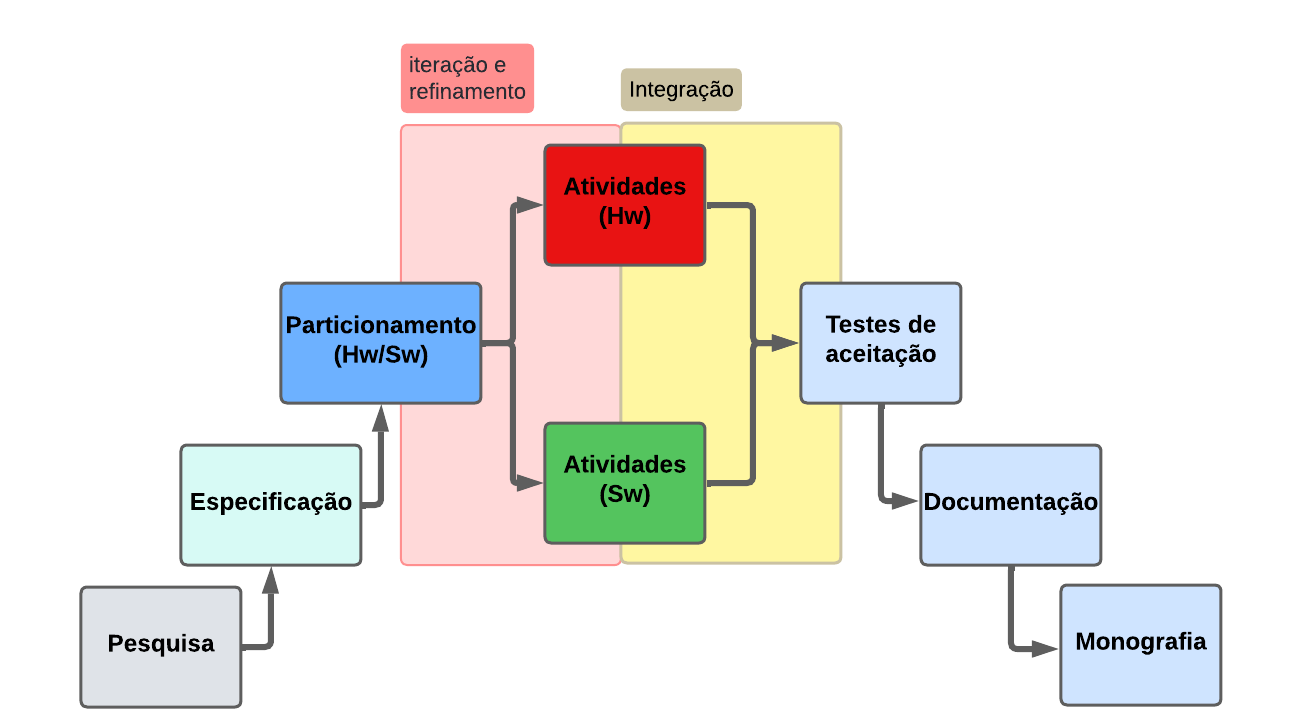
\includegraphics[width=.82\textwidth]{img/diagrama-metodologia.png}
\caption{Fluxo de atividades. Fonte: Elaboração própria com base  em \cite{system-design-IOT}}\label{figMetodologia}
\end{figure}

A primeira fase é a pesquisa. Consiste na busca de trabalhos relacionados na área de sistemas embarcados 
e estudo detalhado dos efeitos do gás monóxido de carbono, em seguida realiza-se a avaliação crítica de cada projeto 
e seus pontos de melhoria. Ao final, ocorre o estudo da medição de concentração do gás, levantamento dos componentes 
eletrônicos para a montagem do protótipo físico e pesquisa com entrevistados sobre as condições físicas do ambiente residencial, pois o
dispositivo deve atender os requisitos do público-alvo.

Em segundo, existe a fase de especificação. Ocorre o levantamento de funcionalidades do sistema, com aplicação de questionário 
e entrevistas para a compreensão do domínio de problema. Por outro lado, é realizada também a modelagem do circuito 
eletrônico, arquitetura do \textit{software} de dados/alerta, fluxo de navegação do aplicativo móvel e, por fim, o 
planejamento da comunicação entre o aplicativo e o dispositivo microcontrolador.

O particionamento em componentes de \textit{hardware} e \textit{software} (Hw/Sw) marca o início do processo iterativo. O terceiro 
processo identifica as funcionalidades do escopo e considera a dependência entre os serviços que as camadas do sistema oferecem. Com isso, 
o fluxo define as atividades necessárias para a entrega da funcionalidade descrita em fases anteriores. Além da definição, a lista de atividades passa 
por um refinamento para eliminar ambiguidade e inconsistência.

A etapa de atividades de \textit{software} e \textit{hardware} foca na simples execução do esboço de sua etapa anterior. Na etapa de integração, os componentes gerados na execução de atividades 
serão submetidos aos casos de teste para verificar o comportamento adequado da entrega parcial, caso contrário os artefatos 
deverão ser revistos para identificar a causa do problema. O ciclo encerra com a finalização de todas as entregas parciais do protótipo.

Os testes de aceitação serão realizados com os usuários finais do sistema. A fase consiste em aplicar questionários para um grupo de pessoas sobre o uso 
do sistema embarcado, considerando dificuldades em configurar o aparelho, uso do aplicativo e leitura dos dados, para, ao final, identificar fatores na interação com o sistema que 
merecem revisão. Em penúltimo, a documentação do sistema é o momento em que todo o projeto será estruturado para o conhecimento da comunidade científica, assim como a confecção do guia 
de uso e instalação. Por fim, a última etapa consiste na escrita da monografia e consolidação dos resultados obtidos com a defesa do trabalho de conclusão de curso.